\documentclass[11pt,a4paper]{article}

% ---------------------------------------------------------------- packages --
\usepackage[margin=1in]{geometry}
\usepackage{lmodern}          % scalable fonts: microtype's expansion needs them
\usepackage[T1]{fontenc}
\usepackage{amsmath,amssymb,amsthm}
\usepackage{graphicx}
\usepackage{booktabs}
\usepackage{microtype}
\usepackage{xcolor}
\usepackage{subcaption}
\usepackage{enumitem}
\usepackage{natbib}
\usepackage{siunitx}
\usepackage[colorlinks=true,linkcolor=blue!50!black,citecolor=blue!50!black,
            urlcolor=blue!50!black]{hyperref}

\graphicspath{{../figures/}}
\bibliographystyle{plainnat}

% ----------------------------------------------------------------- macros ---
\newcommand{\I}{\mathrm{I}}
\newcommand{\HH}{\mathrm{H}}
\newcommand{\R}{\mathbb{R}}
\newcommand{\E}{\mathbb{E}}
\newcommand{\Norm}{\mathcal{N}}
\newcommand{\Wb}{\bar{W}}
\newcommand{\smi}{\sigma_{MI}}
\DeclareMathOperator{\tr}{tr}
\DeclareMathOperator{\STD}{STD}

\newtheorem{claim}{Claim}

\title{\bfseries On the Information Bottleneck Theory of Deep Learning\\
       \large A Reproduction and Critical Study\\[2pt]
       \normalsize after Saxe, Bansal, Dapello, Advani, Kolchinsky, Tracey \& Cox\\
       \normalsize\emph{J.\ Stat.\ Mech.}\ (2019) 124020}
\author{Course project --- Information Theory and Inference}
\date{\today}

\begin{document}
\maketitle

\begin{abstract}
\noindent
The information bottleneck (IB) theory of deep learning makes three claims: that
training passes through a fitting phase followed by a distinct \emph{compression}
phase; that compression causes the good generalisation of deep networks; and that
compression is driven by the diffusion-like noise of stochastic gradient descent.
This report reproduces, from scratch, the analysis of \citet{saxe2019information},
which shows that none of the three survives scrutiny. We implement four mutual
information estimators, validate them against analytic values and against the
original authors' code to a relative accuracy of $10^{-10}$, and re-derive the
paper's results on its own datasets.
Our replication confirms every substantive conclusion. A \texttt{tanh} network
compresses by \SI{10.7}{bits}; changing one identifier to \texttt{relu} reduces
this to \SI{0.5}{bits} while \emph{improving} test accuracy. Holding the network
entirely fixed and changing only the bin edges reduces the deepest layer's
compression from \SI{5.59}{} to \SI{0.32}{bits}. In deep linear networks, where
the mutual information is available in closed form and no estimator is involved,
no compression occurs at all --- and two networks with indistinguishable
information planes differ in generalisation error by a factor of twenty.
Full-batch gradient descent, which contains no stochasticity whatsoever,
compresses \emph{more} than SGD (\SI{17.9}{} versus \SI{10.7}{bits}).
We also report three findings that go beyond the paper: a quantification of
\emph{when} task-irrelevant compression begins (at \SI{39}{\percent} of fitting,
hence interleaved rather than sequential); a demonstration that the Kraskov
estimator is invalid for ReLU layers, whose atom at zero makes
\SI{45}{\percent} of activation vectors identical; and an extension to a small
transformer, where we test whether softmax attention and LayerNorm --- both
bounded operations the paper never examined --- reintroduce artefactual
compression into an architecture built from non-saturating nonlinearities.
\end{abstract}

\tableofcontents
\newpage

% ============================================================================
\section{Introduction}
% ============================================================================

Deep networks work, and it is not settled why. One influential proposal analyses
learning through the lens of information theory
\citep{tishby2015deep,shwartzziv2017opening}. On this view each hidden layer $T$
is a summary statistic of the input $X$, and learning is the search for a
representation that discards as much of $X$ as possible while retaining what
predicts the target $Y$. The natural picture is the \emph{information plane}: a
plot of $\I(T;Y)$ against $\I(X;T)$, one curve per layer, parameterised by
training time.

The appeal is real. Mutual information is architecture-agnostic, so different
models become comparable in a common currency; and the IB principle
\citep{tishby1999information} supplies an optimal frontier against which any
representation can be judged.

\citet{shwartzziv2017opening} reported a striking empirical finding in this
plane: training appears to have two phases --- an initial \emph{fitting} phase in
which $\I(X;T)$ and $\I(T;Y)$ both rise, and a subsequent \emph{compression}
phase in which $\I(X;T)$ falls while $\I(T;Y)$ does not. Three claims were built
on it.

\begin{claim}[Two phases]\label{cl:phases}
Deep network training consists of a fitting phase followed by a distinct
compression phase.
\end{claim}
\begin{claim}[Causality]\label{cl:cause}
The compression phase is causally responsible for good generalisation.
\end{claim}
\begin{claim}[Mechanism]\label{cl:mech}
Compression arises from the diffusion-like behaviour of SGD.
\end{claim}

\citet{saxe2019information} argue that none of the three holds in general, and
that all three reflect assumptions made in order to compute a finite mutual
information at all. This report reproduces their argument from first principles.

\paragraph{What this report contributes.}
Everything is re-implemented from the paper's equations: the networks, the four
estimators, the training instrumentation. We validate each estimator against
analytically known values and, where a reference exists, against the original
authors' code. Beyond replication we (i) quantify the timing of task-irrelevant
compression, which the paper asserts but does not measure; (ii) identify and
diagnose a failure of the Kraskov estimator on ReLU layers that the paper's
appendix does not flag; (iii) document two internal inconsistencies in the
paper's own specification; and (iv) extend the analysis to a transformer.

\paragraph{Deliverables.}
Six Jupyter notebooks (\texttt{01}--\texttt{06}) reproduce the paper section by
section, plus a seventh (\texttt{07}) for the transformer extension. They rest on
a documented library, \texttt{ibdl/}, with a validation suite of 46 checks.

% ============================================================================
\section{Information-theoretic background}
% ============================================================================

\subsection{The information bottleneck principle}

Given jointly distributed $(X,Y)$, the IB problem \citep{tishby1999information}
seeks a stochastic map $p(t \mid x)$ minimising
\begin{equation}
  \mathcal{L}_{\mathrm{IB}} = \I(X;T) - \beta\,\I(T;Y),
  \label{eq:ib}
\end{equation}
trading compression of the input against prediction of the target. Sweeping
$\beta$ traces an optimal frontier in the information plane. For jointly Gaussian
variables the solution is known in closed form \citep{chechik2005information}.

Two structural facts underpin the IB reading of a deep network. First, a
feed-forward network forms a Markov chain
\begin{equation}
  Y \rightarrow X \rightarrow T_1 \rightarrow T_2 \rightarrow \cdots \rightarrow \hat{Y},
\end{equation}
so by the \emph{data processing inequality} (DPI) \citep{cover2006elements}
\begin{equation}
  \I(X;T_1) \ge \I(X;T_2) \ge \cdots, \qquad
  \I(T_1;Y) \ge \I(T_2;Y) \ge \cdots .
  \label{eq:dpi}
\end{equation}
Layers should therefore appear in order along both axes. Second, mutual
information is invariant under invertible reparametrisation, so two networks that
differ only by a change of internal coordinates should be indistinguishable.

Both facts will turn out to fail for the quantity actually plotted --- not
because the theorems are wrong, but because the quantity plotted is not the one
they apply to.

\subsection{The obstruction: deterministic networks carry infinite information}
\label{sec:infinite}

This is the technical heart of the matter. Let a hidden layer compute
$h=f(X)$ with $f$ continuous and deterministic. Then
\begin{equation}
  \I(h;X) = \HH(h) - \HH(h \mid X).
\end{equation}
Given $X$, the activity $h$ is a point mass at $f(X)$; the differential entropy
of a point mass is $-\infty$; hence for any layer with finite $\HH(h)$,
\begin{equation}
  \boxed{\ \I(h;X) = \infty\ }
  \label{eq:infinite}
\end{equation}
at \emph{every} point in training \citep{laughlin1981simple,tishby2015deep}. A
constant cannot have a fitting phase or a compression phase.

Every finite number ever plotted in an information plane is therefore produced by
an additional assumption, of which two are standard:
\begin{enumerate}[label=(\roman*),topsep=2pt,itemsep=1pt]
  \item \textbf{Binning.} Discretise $h$ into $T=\mathrm{bin}(h)$. Then $T$ is a
    deterministic function of $X$ but discrete, so $\HH(T \mid X)=0$ and
    $\I(T;X)=\HH(T)$ is finite.
  \item \textbf{Added noise.} Define $T=h+Z$ with $Z \perp X$. Then
    $\HH(T \mid X) = \HH(Z)$ is finite, so $\I(T;X) = \HH(T)-\HH(Z)$ is finite.
\end{enumerate}
Neither is part of the network. Both are choices made by the analyst, and
\emph{the trajectory reports on the choice as much as on the network}. This is
the thesis of the paper and the organising idea of this report.

Two consequences follow immediately and are worth stating, because they undercut
the two structural facts above.

\paragraph{The DPI does not apply.} Noise added post hoc at each layer does not
propagate. For $X \to h_1 \to h_2$ with analysis variables $T_i = h_i + Z_i$, the
chain is $X \to h_1 \to h_2 \to T_2$, not $X\to h_1 \to T_1 \to T_2$. The DPI
therefore bounds $\I(X;h_1) \ge \I(X;T_2)$ and says nothing about
$\I(X;T_1)$ versus $\I(X;T_2)$. Apparent DPI violations in published information
planes are artefacts of this.

\paragraph{Invariance is destroyed.} $T = h+Z$ is not invariant under
reparametrisation of $h$, because the noise enters at a fixed scale. We give a
concrete demonstration in \S\ref{sec:rescale}.

\subsection{The four estimators}
\label{sec:estimators}

We implement all four routes to a finite number used in the paper. Each is
defined below and validated in \S\ref{sec:validation}.

\paragraph{(1) Binning.} With the input alphabet finite and fully enumerated, and
taken uniform,
\begin{equation}
  \I(T;X) = \HH(T) - \underbrace{\HH(T \mid X)}_{=0} = -\sum_i p_i \log p_i,
  \label{eq:binning}
\end{equation}
where $p_i$ is the probability that an input lands in bin $i$. For a monotone
nonlinearity and scalar Gaussian input this is exact via the Gaussian CDF,
\begin{equation}
  p_i = \Phi\!\big(f^{-1}(b_{i+1})/w_1\big) - \Phi\!\big(f^{-1}(b_{i})/w_1\big).
  \label{eq:bincdf}
\end{equation}
The label $Y$ is genuinely discrete, so
$\I(T;Y)=\HH(T)-\sum_y p(y)\HH(T\mid Y{=}y)$ needs no further assumption.

\paragraph{(2) Kernel density bounds.} Assume $T=h+\epsilon$,
$\epsilon\sim\Norm(0,\sigma^2 I)$, and take the empirical input distribution.
Then $p(T)$ is \emph{exactly} a uniform mixture of $P$ Gaussians centred at the
$h_i$, and pairwise distances bound its entropy
\citep{kolchinsky2017estimating}. Since $\HH(T\mid X)=\HH(\epsilon)$,
\begin{equation}
  \I(T;X) \;\le\; -\frac{1}{P}\sum_i \log \frac{1}{P}\sum_j
    \exp\!\left(-\frac{1}{2}\frac{\lVert h_i-h_j\rVert_2^2}{\sigma^2}\right),
  \label{eq:kdeupper}
\end{equation}
with the Bhattacharyya lower bound obtained by replacing $\sigma^2 \to 4\sigma^2$
inside the exponent. The normalising constants cancel exactly --- a useful check
on the algebra.

\paragraph{(3) Kraskov $k$-NN.} If $T=h+Z$ with $Z\perp X$ then
$\I(T;X)=\HH(T)-\HH(Z)=\HH(T)-c$ for a \emph{constant} $c$, so compression can be
read off $\HH(T)$ alone without fixing a noise level. The
Kozachenko--Leonenko estimator \citep{kozachenko1987sample,kraskov2004estimating}
gives
\begin{equation}
  \hat{\HH} = \frac{d}{P}\sum_{i=1}^{P}\log(r_i+\varepsilon)
    + \frac{d}{2}\log\pi - \log\Gamma(d/2+1) + \psi(P) - \psi(k),
  \label{eq:kraskov}
\end{equation}
with $r_i$ the distance to the $k$-th nearest neighbour. We show in
\S\ref{sec:kraskovfail} that this estimator is \emph{invalid} for ReLU layers.

\paragraph{(4) Exact linear--Gaussian.} For a deep linear network with
$X\sim\Norm(0,\Sigma_X)$, a hidden layer applying the cumulative map
$\Wb = W_l\cdots W_1$, and analysis noise $\smi$,
\begin{align}
  \I(T;X) &= \tfrac12 \log\big|\Wb\Sigma_X\Wb^\top + \smi^2 I\big|
           - \tfrac12 \log\big|\smi^2 I\big|,
  \label{eq:exactx}\\
  \I(T;Y) &= \HH(T)+\HH(Y)-\HH(T,Y),
  \label{eq:exacty}
\end{align}
all in closed form. This estimator has \emph{no error}, which makes it decisive.

\paragraph{Subspace information.} For \S\ref{sec:simul} we need the information a
layer carries about a \emph{subset} $S$ of input coordinates. Conditioning on
$X_S$ leaves the complement acting as noise:
\begin{equation}
  \I(T;X_S) = \tfrac12\log\big|\Wb\Sigma_X\Wb^\top+\smi^2 I\big|
    - \tfrac12\log\big|\Wb_{\bar S}\Sigma_{\bar S}\Wb_{\bar S}^\top + \smi^2 I\big|.
  \label{eq:subspace}
\end{equation}
Since $X_{\mathrm{rel}} \perp X_{\mathrm{irrel}}$, the chain rule gives
\begin{equation}
  \I(X;T) = \I(X_{\mathrm{rel}};T) + \I(X_{\mathrm{irrel}};T)
          + \underbrace{\I(X_{\mathrm{rel}};X_{\mathrm{irrel}} \mid T)}_{\ge 0},
  \label{eq:subadd}
\end{equation}
so the parts are \emph{sub-additive}: observing $T$ makes two a priori
independent blocks dependent (``explaining away''). We use this in
\S\ref{sec:simul} to explain how $\I(X_{\mathrm{irrel}};T)$ can fall while
$\I(X;T)$ rises.

% ============================================================================
\section{Methods and validation}
% ============================================================================

\subsection{Datasets and architectures}

\paragraph{The 12-bit dataset.} The synthetic dataset of
\citet{shwartzziv2017opening}: all $2^{12}=4096$ twelve-bit patterns, each
appearing exactly once, with a binary label ($P(Y{=}1)=0.517$, so
$\HH(Y)=\SI{0.9992}{bits}$). We use the authors' own \texttt{var\_u.mat}. The
crucial property is that the input alphabet is \emph{finite and fully
enumerated}: taking it uniform gives $\HH(X)=\log_2 4096 = \SI{12}{bits}$
exactly, and binning-based mutual information evaluated over all 4096 patterns
has \emph{no sampling error}. The network is
$12$--$10$--$7$--$5$--$4$--$3$--$2$, the last layer two sigmoidal units, trained
by SGD on \SI{80}{\percent} of the patterns with 256 samples per batch.

\paragraph{Linear student--teacher.} $X\sim\Norm(0,I/N_i)$,
$Y = W_o X + \epsilon_o$ with $W_{o,ij}\sim\Norm(0,\sigma_w^2)$ and
$\epsilon_o\sim\Norm(0,\sigma_o^2)$; $\mathrm{SNR}=\sigma_w^2/\sigma_o^2$. The
student is a deep linear network. The exact generalisation error is
\begin{equation}
  E_g = \tr\!\big[(W_o-W_{\mathrm{tot}})\Sigma_X(W_o-W_{\mathrm{tot}})^\top\big]
        + \sigma_o^2 N_o .
  \label{eq:eg}
\end{equation}

\paragraph{MNIST.} $784$--$1024$--$20$--$20$--$20$--$10$, SGD with minibatches of
128. The three narrow layers are the paper's choice, made so the kernel density
estimator stays well conditioned.

\subsection{Two inconsistencies in the paper's specification}
\label{sec:inconsistencies}

Reproducing the paper exactly required resolving two internal conflicts. We
record them because they affect any attempt to reproduce this work.

\paragraph{(i) Missing $\Sigma_X$ and a missing factor of $\tfrac12$.} The text
states $X\sim\Norm(0,\tfrac{1}{N_i}I_{N_i})$, but equations~(5), (6) and
(G.1)--(G.3) are written with $\Sigma_X$ suppressed, as though $\Sigma_X=I$;
and equation~(6) additionally drops the factor $\tfrac12$ that appears correctly
in~(G.2). We carry both explicitly, as in \eqref{eq:exactx} and \eqref{eq:eg}.
This is a constant offset and a scale on the axes, not a change to any
conclusion; and it places $\I(X;T)$ in the range $0.5$--\SI{2.5}{bits}, matching
the axes of the paper's own figure~3D.

\paragraph{(ii) Figures 3 and 4 are described identically but conclude
oppositely.} Figure~3 (``generalises well, minimal overtraining'') and figure~4
(``overfitting is substantial'') are both specified with $N_i = P = 100$ and one
hidden layer of 100 units. Since \citet{advani2017high} --- cited by the paper
for exactly this point --- show overtraining is \emph{worst} at $P=N_i$, the two
cannot differ in the stated parameters. We determined empirically that the
distinguishing factor is the optimiser and the training horizon: figure~3 is
batch gradient descent over 500 epochs (its colour bar tops out at epoch 499),
figure~4 is SGD with 5 samples per batch, i.e.\ 20 updates per epoch. With that
reading both regimes reproduce cleanly.

\subsection{Estimator validation}
\label{sec:validation}

Because the entire argument rests on the estimators, we validate them before
using them. Table~\ref{tab:validation} summarises; all 46 checks pass.

\begin{table}[t]
\centering
\small
\begin{tabular}{llr}
\toprule
\textbf{Estimator} & \textbf{Check} & \textbf{Result} \\
\midrule
Binning  & $P$ distinct patterns $\Rightarrow \I=\log_2 P$ & exact to $10^{-12}$ \\
Binning  & $T=Y \Rightarrow \I(T;Y)=\HH(Y)$ & exact to $10^{-12}$ \\
Binning  & vs.\ authors' \texttt{simplebinmi.py} & $10^{-10}$ relative \\
KDE      & vs.\ authors' \texttt{kde.py} & $10^{-10}$ relative \\
KDE      & bounds bracket Gaussian channel value & $3.69 \le 3.99 \le 4.69$ \\
KDE      & chunked vs.\ unchunked evaluation & identical (0.0) \\
Kraskov  & $\HH(U[0,1]^d)=0$, $d=1,2,3$ & $|\hat{\HH}| < 0.03$ nats \\
Kraskov  & $\HH(\Norm(0,\sigma^2I_2))$ & within 0.008 nats \\
Kraskov  & $\HH(cX)=\HH(X)+d\log c$ & exact to $10^{-6}$ \\
Exact    & scalar channel $\tfrac12\log_2(1+w^2/\smi^2)$ & exact to $10^{-12}$ \\
Exact    & parallel channels add & exact to $10^{-12}$ \\
Exact    & DPI holds when noise is propagated & confirmed \\
Exact    & sub-additivity \eqref{eq:subadd}, synergy $\ge 0$ & confirmed \\
Cross    & exact value lies within KDE bounds & $1.38 \le 2.08 \le 3.45$ \\
Cross    & Kraskov $\hat{\HH}(T)$ vs.\ exact Gaussian $\HH(T)$ & within 0.01 bits \\
Trainers & NumPy linear vs.\ PyTorch autograd & $10^{-7}$, $17\times$ faster \\
Trainers & \texttt{vmap} per-sample grads vs.\ loop & $10^{-9}$ \\
\bottomrule
\end{tabular}
\caption{Validation of the estimators and trainers. Agreement with the original
authors' implementations is to relative $10^{-10}$; agreement with analytically
known values is to the precision of the estimator.}
\label{tab:validation}
\end{table}

\subsection{Instrumentation}

Per-sample gradients for the SNR statistics of equations~(I.1)--(I.2),
\begin{equation}
  m_l = \Big\lVert \big\langle \partial E/\partial W_l\big\rangle \Big\rVert_F,
  \qquad
  s_l = \Big\lVert \STD\big(\partial E/\partial W_l\big) \Big\rVert_F,
  \qquad
  \mathrm{SNR}_l = m_l/s_l,
  \label{eq:snr}
\end{equation}
are computed with \texttt{torch.func.vmap(grad(...))} in a single vectorised
pass, accumulated in Welford form so memory stays $O(\text{params})$ rather than
$O(P\cdot\text{params})$. For MNIST, where per-sample gradients over
\num{825390} parameters do not fit, we use the paper's alternative protocol and
take statistics across SGD minibatches.

% ============================================================================
\section{Compression is a property of the nonlinearity}
% ============================================================================

\subsection{An exactly solvable model}

Consider the minimal network of the paper's figure~2: a scalar Gaussian input, a
single weight, a nonlinearity, and binning,
\begin{equation}
  X \sim \Norm(0,1), \qquad h = f(w_1 X), \qquad T = \mathrm{bin}(h).
\end{equation}
Equations~\eqref{eq:binning}--\eqref{eq:bincdf} give $\I(T;X)$ \emph{exactly}: no
sampling, no estimator. Figure~\ref{fig:minimal} shows the result.

\begin{figure}[t]
\centering
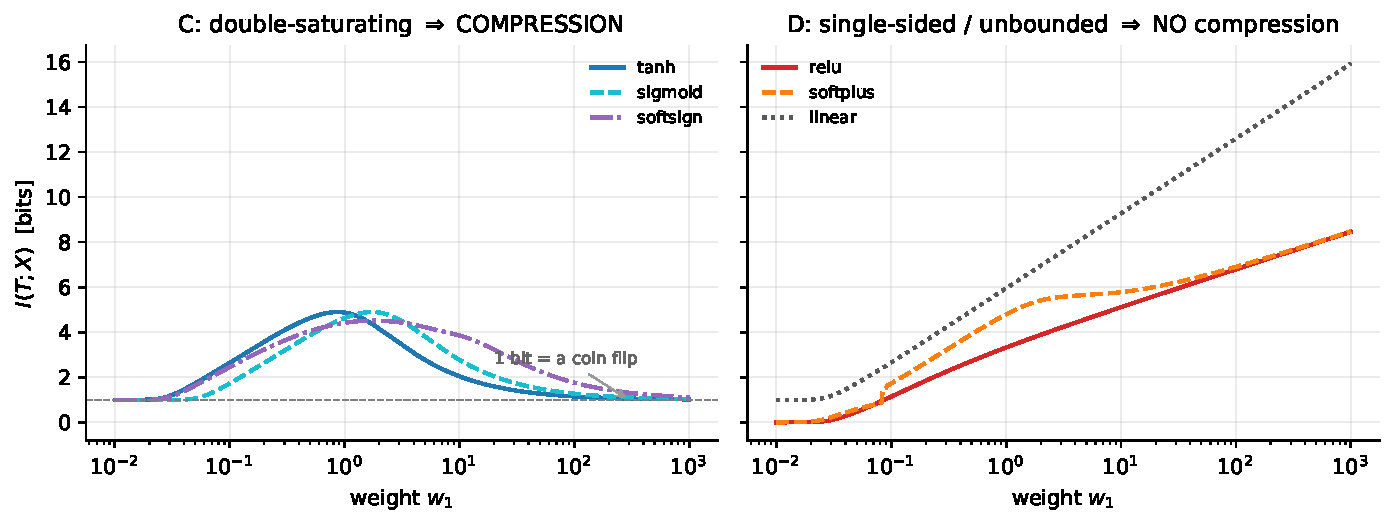
\includegraphics[width=\linewidth]{fig02CD_minimal_model.pdf}
\caption{Exact $\I(T;X)$ versus weight magnitude in the minimal model.
\textbf{Left:} double-saturating nonlinearities rise, peak, and fall back to
exactly \SI{1}{bit} --- for large $w_1$ almost every input saturates into one of
the two extreme bins, leaving only the sign of the input, a single coin flip.
\textbf{Right:} single-sided and unbounded nonlinearities rise without bound.
Both panels use identical machinery; only the shape of $f$ differs.}
\label{fig:minimal}
\end{figure}

The asymptotic slopes are themselves informative: the linear unit gains
$\log_2 10 = \SI{3.32}{bits}$ per decade of $w_1$, and ReLU gains exactly half of
that, \SI{1.66}{bits}, because half of its input distribution lands in the zero
bin and only the positive half spreads out. Our measurements reproduce both to
three decimals.

Since networks are initialised with small weights and \emph{must} grow them to
compute anything nonlinear (a \texttt{tanh} network with tiny weights is confined
to its linear regime), a \texttt{tanh} network traverses the left panel from left
to right during training. \emph{That traversal is the reported compression
phase.}

\subsection{The full network}

Figure~\ref{fig:plane} shows the information plane for the
$12$--$10$--$7$--$5$--$4$--$3$--$2$ network. The \texttt{tanh} result replicates
\citet{shwartzziv2017opening}; the ReLU result does not compress.

\begin{figure}[t]
\centering
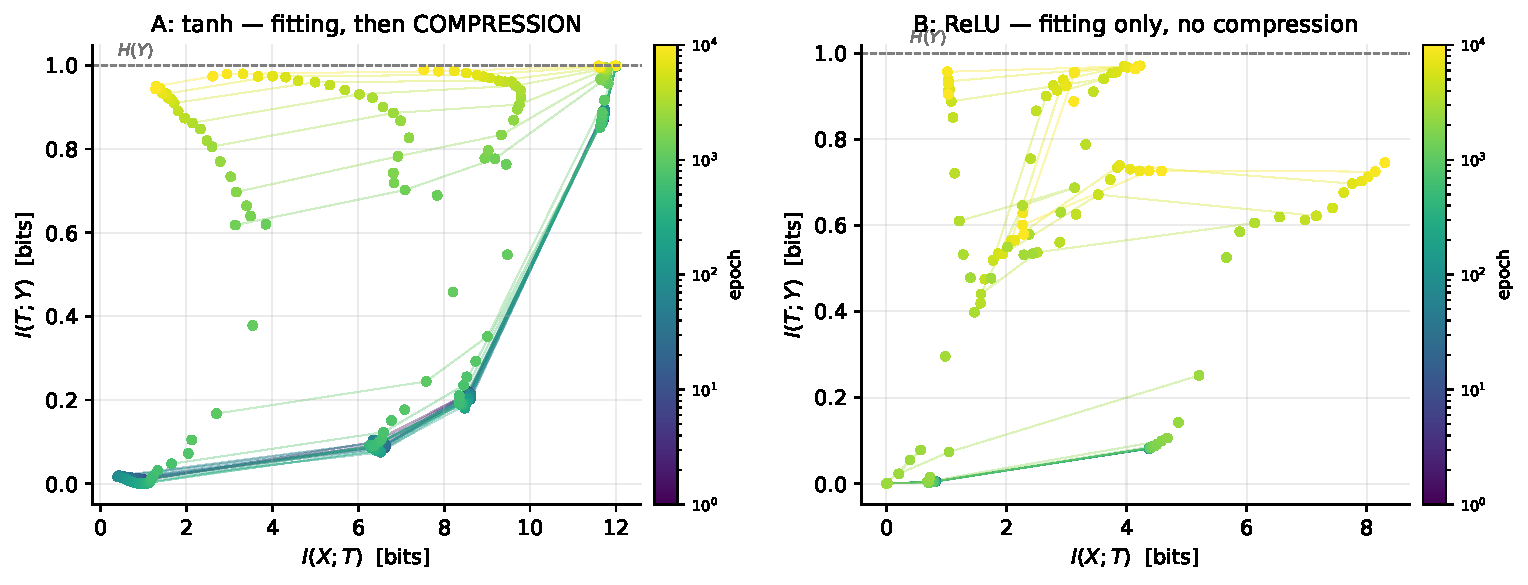
\includegraphics[width=\linewidth]{fig01AB_information_plane.pdf}
\caption{Information plane, binning estimator, all 4096 patterns.
\textbf{A:} \texttt{tanh} --- fitting followed by compression, replicating the
original result. \textbf{B:} ReLU --- fitting only. The only ReLU curve that
compresses is the output layer, which is still sigmoidal.}
\label{fig:plane}
\end{figure}

\begin{table}[t]
\centering
\small
\begin{tabular}{lrrrrrrr}
\toprule
& \multicolumn{6}{c}{compression per layer (bits lost from peak $\I(X;T)$)} & \\
\cmidrule(lr){2-7}
\textbf{network} & L1 & L2 & L3 & L4 & L5 & L6 (out) & \textbf{total} \\
\midrule
\texttt{tanh}, SGD & 0.00 & 0.02 & 0.23 & 2.27 & \textbf{5.59} & 2.56 & \textbf{10.66} \\
\texttt{tanh}, BGD & 0.01 & 1.34 & 3.30 & 3.86 & \textbf{6.52} & 2.84 & \textbf{17.87} \\
ReLU, SGD          & 0.00 & 0.00 & 0.00 & 0.02 & 0.08 & 0.37 & 0.47 \\
ReLU, BGD          & 0.00 & 0.00 & 0.00 & 0.03 & 0.11 & 0.00 & 0.13 \\
\bottomrule
\end{tabular}
\caption{Compression by activation function and optimiser. The \texttt{tanh}
network compresses more than twenty times as much as the ReLU network --- and
compresses \emph{more} under fully deterministic batch gradient descent than
under SGD, contradicting Claim~\ref{cl:mech}.}
\label{tab:compression}
\end{table}

The two networks reach comparable accuracy (\SI{96.2}{\percent} versus
\SI{97.3}{\percent} test), so the difference is not a difference in learning
success. The mechanism is visible directly in the activations: in the
\texttt{tanh} network the fraction of layer-5 units in saturation
($|h|>0.98$) rises from \SI{0.0}{\percent} to \SI{75.4}{\percent} over training,
while ReLU activations disperse without bound (maximum activity \num{56.3}).

\subsection{The measurement, not the network}
\label{sec:binningchoice}

If compression were a property of the network, it would not move when we change
the analysis. It moves. Holding the trained network, its weights and its entire
training history \emph{completely fixed}, and changing only the bin edges from
evenly spaced in activation to evenly spaced in net input,
$b_i \in \tanh(\mathrm{linspace}(-50,50,N))$, gives
Figure~\ref{fig:binningchoice}: layer 5's compression falls from \SI{5.59}{} to
\SI{0.32}{bits}.

\begin{figure}[t]
\centering
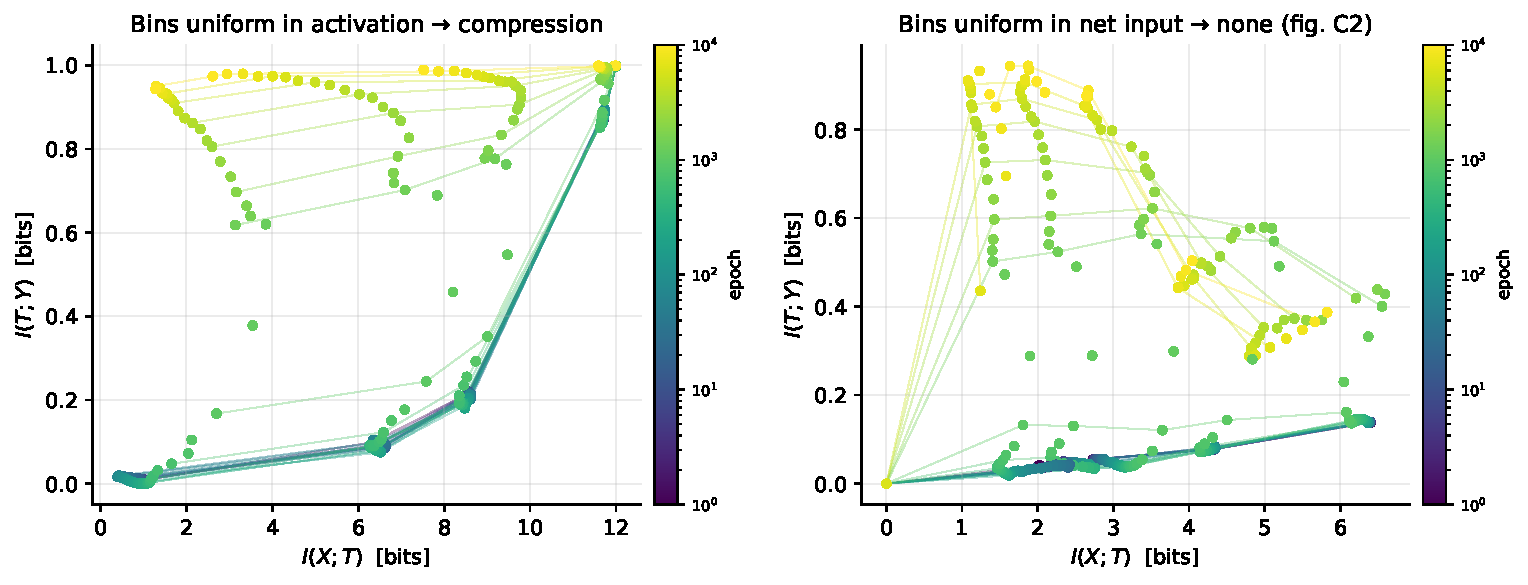
\includegraphics[width=\linewidth]{figC2_binning_changes_conclusion.pdf}
\caption{The same network, the same weights, the same training run --- measured
with two different sets of bin edges. Compression appears or disappears
according to the analyst's choice.}
\label{fig:binningchoice}
\end{figure}

Resolution matters as much as placement. At full machine precision every one of
the 4096 patterns receives its own code and $\I(X;T)$ is pinned at
$\log_2 4096 = \SI{12}{bits}$ with essentially no dynamics --- and a real network
on real hardware is nearer that regime ($\sim 2^{32}$ levels per unit) than the
30 bins used here.

\subsection{Robustness across estimators, and a failure}
\label{sec:kraskovfail}

The KDE bounds confirm the split and refine it (Table~\ref{tab:kde}):
\texttt{softsign} is double-saturating but approaches its asymptotes more gently
than \texttt{tanh}, and compresses correspondingly less; \texttt{softplus} is a
smoothed ReLU and behaves like one. The ordering tracks saturation, not anything
about the optimiser.

\begin{table}[h]
\centering
\small
\begin{tabular}{lcc}
\toprule
\textbf{activation} & \textbf{double-saturating?} & \textbf{max compression (bits)} \\
\midrule
\texttt{tanh}     & yes & 0.69 \\
\texttt{softsign} & yes & 0.11 \\
\texttt{relu}     & no  & 0.10 \\
\texttt{softplus} & no  & 0.01 \\
\bottomrule
\end{tabular}
\caption{KDE estimator, mean of five seeds. Compression tracks saturation
behaviour.}
\label{tab:kde}
\end{table}

\paragraph{The Kraskov estimator is invalid for ReLU.} This is a finding beyond
the paper. Applying \eqref{eq:kraskov} to our ReLU layers returns entropies as
low as $-\SI{88}{bits}$, far below the $\log_2 4096 = \SI{12}{bit}$ ceiling any
genuine entropy here must respect. The cause: a ReLU unit that is off outputs
\emph{exactly} zero, so \SI{44.6}{\percent} of ReLU activation vectors are
bit-identical (versus \SI{0}{\percent} for \texttt{tanh}). The distribution has an
\emph{atom} at zero, making it mixed discrete--continuous, for which differential
entropy is not defined; Kozachenko--Leonenko assumes absolute continuity.
Operationally, when $r_i=0$ the guard $\varepsilon$ takes over and each duplicated
point contributes $(d/P)\log\varepsilon \approx -36.8\,d/P$ nats, so the estimate
reports \emph{how many points coincide}. The paper introduces
$\varepsilon=10^{-16}$ to ``prevent infinite terms'' without noting that the
estimate is then meaningless. We therefore read the \texttt{tanh} panel --- which
agrees with the other estimators, layers 4 and 5 losing \SI{8.5}{} and
\SI{21.3}{bits} --- and discard the ReLU panel.

% ============================================================================
\section{Exact information in deep linear networks}
% ============================================================================

The results so far could in principle be blamed on estimation. Deep linear
networks remove that possibility: every hidden layer is jointly Gaussian with
input and output, so \eqref{eq:exactx}--\eqref{eq:exacty} are exact. They also
answer a second objection --- that compression might come from neurons becoming
correlated or from irrelevant directions being projected out, neither visible in
a one-neuron model.

\begin{figure}[t]
\centering
\begin{subfigure}{\linewidth}
  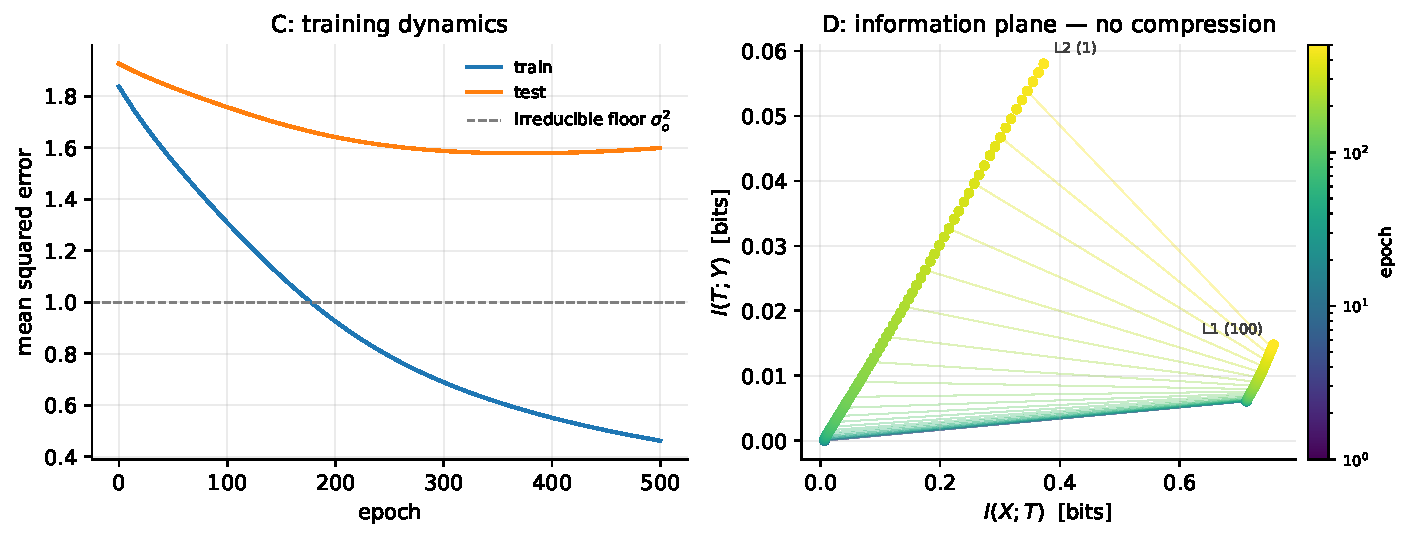
\includegraphics[width=\linewidth]{fig03CD_linear_bgd.pdf}
  \caption{Batch gradient descent, 500 epochs: generalises well.}
\end{subfigure}\\[4pt]
\begin{subfigure}{\linewidth}
  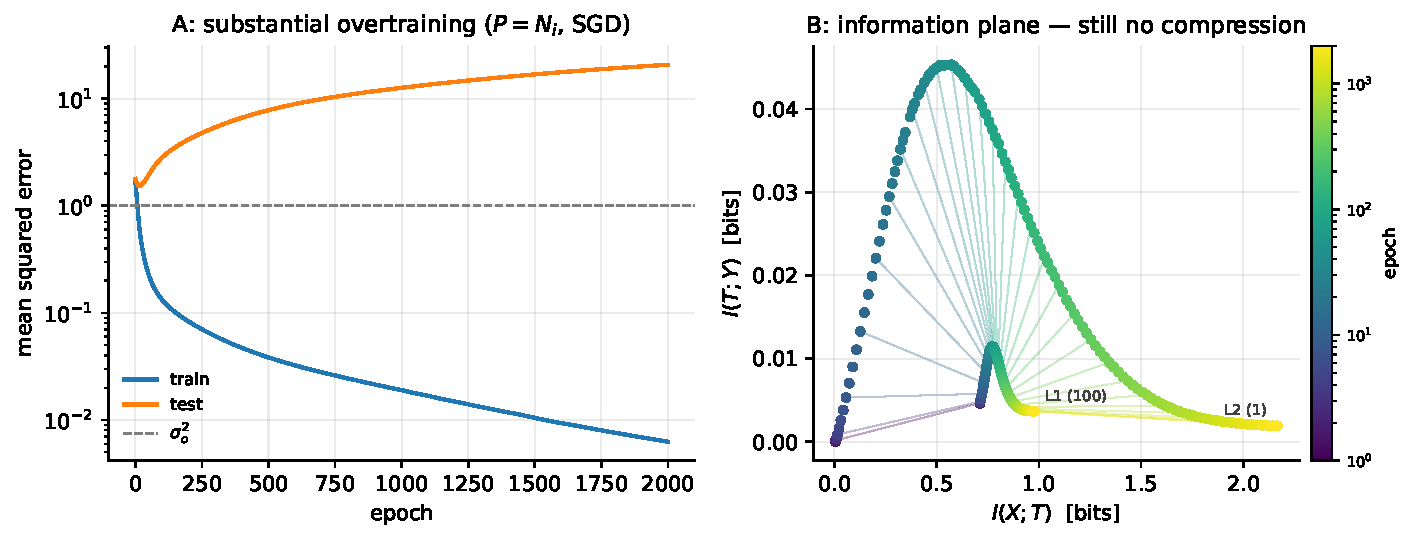
\includegraphics[width=\linewidth]{fig04AB_linear_overfit.pdf}
  \caption{SGD, 5 samples per batch: overfits by a factor of 13.5.}
\end{subfigure}
\caption{Exact information planes in deep linear networks. The two settings have
identical architecture and data-generating process and \emph{indistinguishable}
information planes --- both monotonically increasing, neither compressing --- yet
their generalisation differs by more than an order of magnitude.}
\label{fig:linear}
\end{figure}

No compression occurs in any layer, at any depth, under SGD or BGD, over 500
epochs or \num{20000}. The largest single-step decrease anywhere is
$\sim 10^{-5}$ bits, four orders of magnitude below the overall rise, and no
layer ever ends below its peak.

\subsection{The dissociation}

Table~\ref{tab:dissoc} collects every configuration. If Claim~\ref{cl:cause} held,
the ``compresses'' and ``generalises'' columns would agree. All four combinations
occur.

\begin{table}[h]
\centering
\small
\begin{tabular}{lrcrc}
\toprule
\textbf{network} & \textbf{compression} & \textbf{compresses?}
                 & \textbf{gap / $E_g$ ratio} & \textbf{generalises?} \\
\midrule
\texttt{tanh}, \SI{80}{\percent} data & \SI{10.66}{bits} & yes & 0.019 & yes \\
ReLU, \SI{80}{\percent} data          & \SI{0.47}{bits}  & no  & 0.014 & yes \\
\texttt{tanh}, \SI{30}{\percent} data & \SI{7.99}{bits}  & yes & 0.063 & no  \\
ReLU, \SI{30}{\percent} data          & \SI{0.62}{bits}  & no  & 0.055 & no  \\
\midrule
linear, BGD (fig.\ 3)                 & \SI{0.00}{bits}  & no  & $1.6\times$ & yes \\
linear, SGD $b{=}5$ (fig.\ 4)         & \SI{0.00}{bits}  & no  & $20.3\times$ & no \\
\bottomrule
\end{tabular}
\caption{Compression and generalisation vary independently. Neither implies the
other, refuting Claim~\ref{cl:cause}.}
\label{tab:dissoc}
\end{table}

\subsection{Identical functions, different information}
\label{sec:rescale}

The sharpest illustration that the measured quantity is not a property of the
function computed. Take $\hat{y}=w_2w_1x$ and rescale
$\tilde{w}_1 = w_1/c$, $\tilde{w}_2 = c\,w_2$. Every member of this family
computes \emph{exactly the same map} and so generalises identically. But
\begin{equation}
  \I(T;X) = \tfrac12\log\big(w_1^2/c^2+\smi^2\big) - \tfrac12\log\smi^2,
  \label{eq:c5}
\end{equation}
which depends on $c$: from \SI{4.32}{bits} at $c=0.1$ down to \SI{0.03}{bits} at
$c=10$, for an unchanged input--output map. Mutual information is invariant under
invertible reparametrisation; $T=h+Z$ is not, because the noise enters at a fixed
scale.

% ============================================================================
\section{Compression is not caused by SGD noise}
% ============================================================================

Claim~\ref{cl:mech} states that compression arises from the diffusion phase of
SGD. It fails on two independent grounds.

\paragraph{Theoretically.} The argument runs: diffusion drives the weight
distribution to maximum entropy subject to a training-error constraint; maximum
entropy maximises $\HH(X\mid T)$; hence $\I(X;T)=\HH(X)-\HH(X\mid T)$ is
minimised. The middle step does not follow. The maximum-entropy distribution is
over \emph{weights across training runs}; $\HH(X\mid T)$ is uncertainty about
\emph{inputs drawn from the data distribution, given one fixed network}. These
are different random variables, and there is no general reason a sample from the
former maximises the latter.

\paragraph{Empirically.} The claim makes a testable prediction: remove the
randomness and compression should vanish. Full-batch gradient descent has no
sampling noise and no diffusion. Table~\ref{tab:compression} shows \texttt{tanh}
compression under BGD is \SI{17.9}{bits} --- \emph{larger} than the
\SI{10.7}{bits} under SGD. The prediction fails in the wrong direction.

\paragraph{The SNR transition is real but unrelated.} Both networks lose one to
two orders of magnitude of gradient SNR over training (\numrange{20}{68}$\times$
per layer), with no systematic difference between the compressing and
non-compressing network. The transition is a property of \emph{arriving at a
minimum}: the mean gradient vanishes there by definition, while per-sample
disagreement does not. It was described long before the IB literature as the
transient/stochastic phases \citep{murata1998statistical}.

The decisive case is a $1$--$1$--$1$ linear network with small initial weights
(Figure~\ref{fig:i2}). With a single hidden unit whose weight only grows,
compression is impossible \emph{by construction} --- yet the SNR falls by a
factor of \num{16502}.

\begin{figure}[t]
\centering
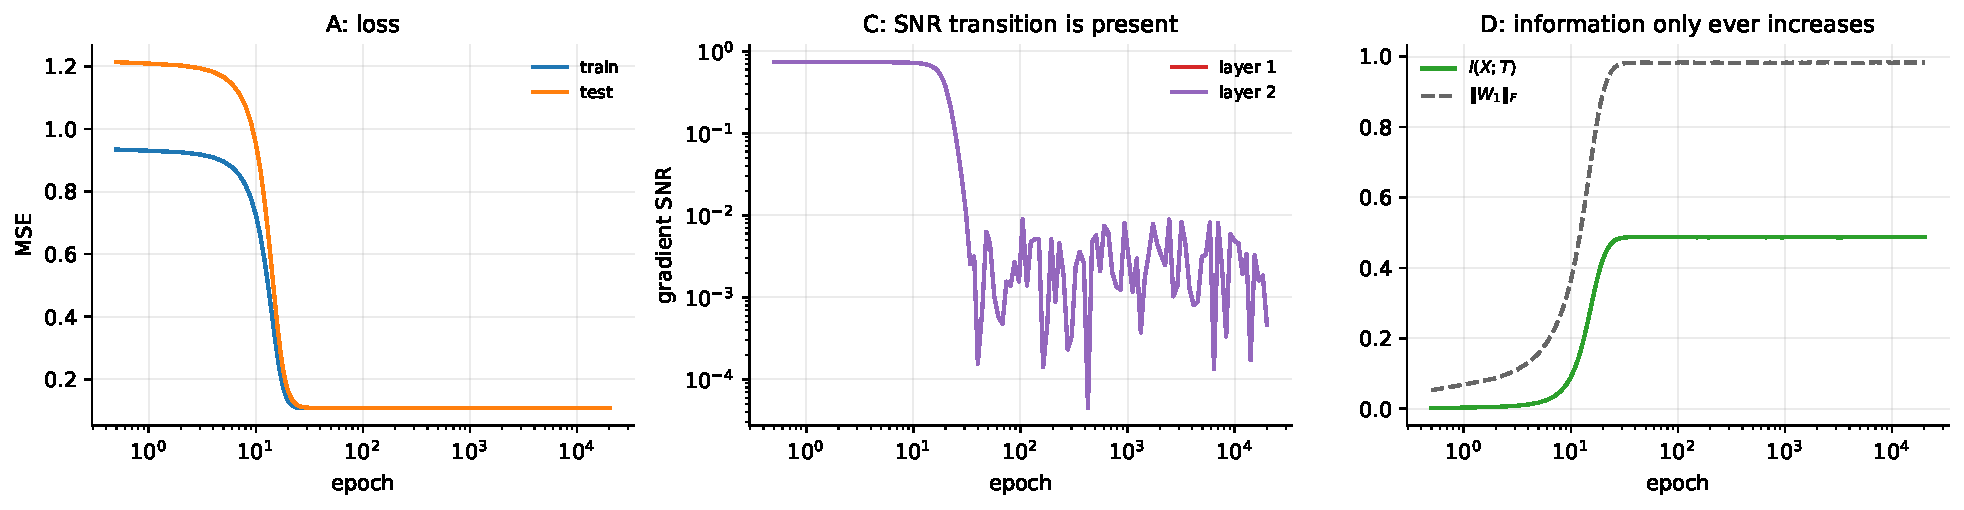
\includegraphics[width=\linewidth]{figI2_minimal_snr.pdf}
\caption{A $1$--$1$--$1$ linear network. The gradient SNR undergoes a textbook
drift$\to$diffusion collapse ($\num{16502}\times$) while the weight norm
\emph{grows} and $\I(X;T)$ only ever increases. The SNR transition is therefore
independent of compression.}
\label{fig:i2}
\end{figure}

% ============================================================================
\section{When compression does occur --- and when}
\label{sec:simul}
% ============================================================================

One intuition survives all of the above: if some input channels carry only noise,
good generalisation \emph{requires} discarding them. The paper takes this
seriously, partitioning the input into a task-relevant block and a
task-irrelevant block with the teacher's weights on the latter set to exactly
zero. Using \eqref{eq:subspace}, everything is again exact.

\begin{figure}[t]
\centering
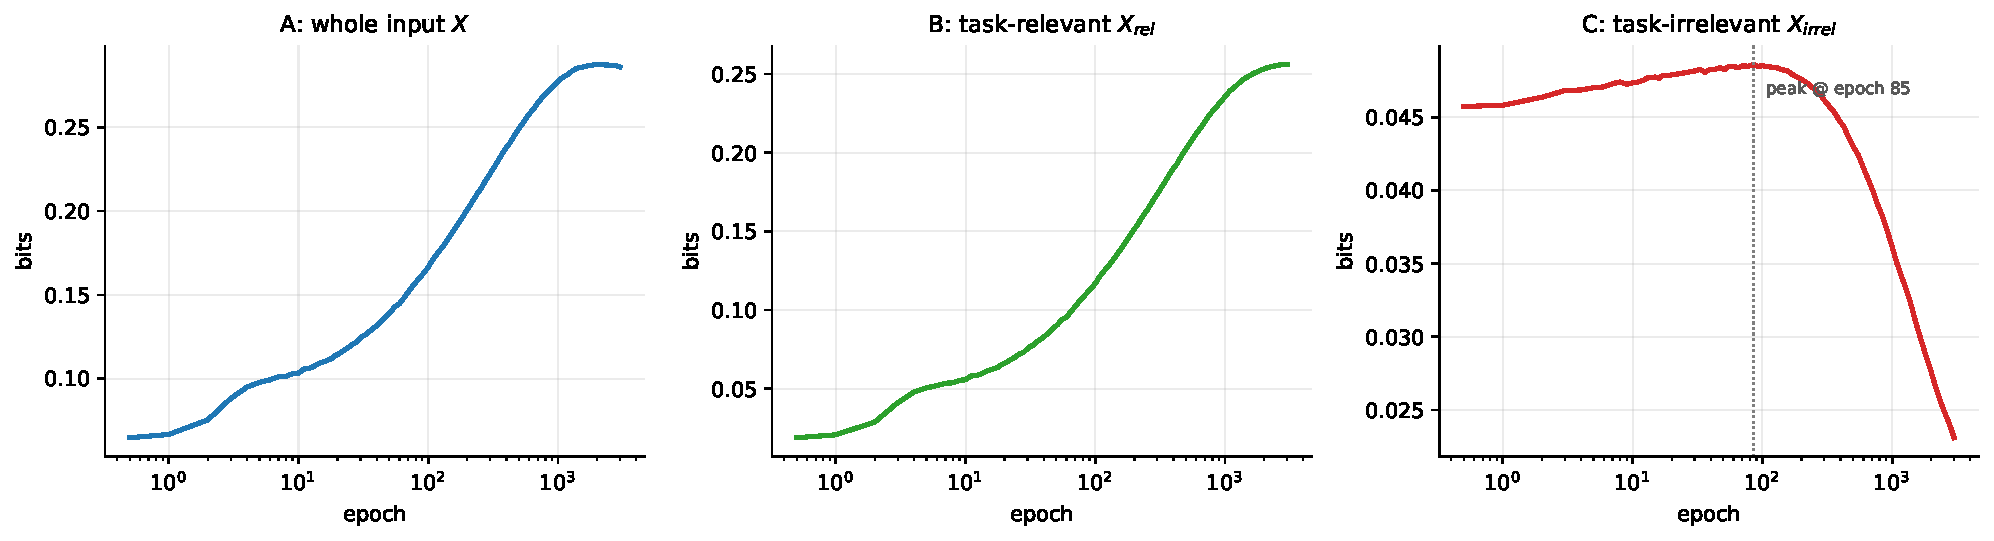
\includegraphics[width=\linewidth]{fig06_simultaneous.pdf}
\caption{\textbf{A:} information about the whole input does \emph{not} compress.
\textbf{B:} information about the relevant subspace rises robustly.
\textbf{C:} information about the irrelevant subspace rises and then falls ---
genuine compression, invisible in panel A.}
\label{fig:simul}
\end{figure}

So the intuition is half right. $\I(X_{\mathrm{irrel}};T)$ peaks at
\SI{0.049}{bits} and falls to \SI{0.023}{bits}, a \SI{53}{\percent} reduction,
while $\I(X;T)$ rises throughout. The sub-additivity identity \eqref{eq:subadd}
explains the apparent paradox: the synergy term
$\I(X_{\mathrm{rel}};X_{\mathrm{irrel}}\mid T)\ge 0$ absorbs the difference. We
verify numerically that this term is non-negative throughout.

\paragraph{The timing.} The IB claim is not merely that compression happens but
that it occupies a \emph{separate second phase}. The paper asserts the two are
concurrent; we quantify it. Compression of the irrelevant subspace begins at
epoch 85, at which point fitting of the relevant subspace is only
\SI{39}{\percent} complete (\SI{33}{\percent} and \SI{7}{\percent} for two other
seeds). Fitting reaches \SI{90}{\percent} completion only at epoch 995, more than
ten times later. \textbf{The two processes are interleaved, not sequential.}

\paragraph{Consequence for methodology.} The compression that a task actually
demands is invisible in $\I(X;T)$, the quantity the standard information plane
plots. Detecting it requires a subspace-resolved measure. This is a positive
finding: the information-theoretic framing is not useless, but the aggregate
statistic is the wrong instrument.

% ============================================================================
\section{Extension: does a transformer compress?}
% ============================================================================

The paper's mechanism is stated for the activation function, and modern
architectures use non-saturating ones. But a transformer block contains two
operations the paper never examined, both \emph{bounded}:
\begin{itemize}[topsep=2pt,itemsep=1pt]
  \item \textbf{softmax attention} \citep{vaswani2017attention}: each output is a
    convex combination of value vectors, confined to their convex hull, and the
    attention weights themselves saturate towards one-hot as logits grow;
  \item \textbf{LayerNorm} \citep{ba2016layer}: projects the residual stream onto
    a sphere of fixed radius $\sqrt{d}$, so however large the weights grow the
    representation cannot spread.
\end{itemize}
Both saturate in the relevant sense. The paper's own mechanism therefore predicts
that a transformer should exhibit apparent compression driven by its
\emph{normalisation and attention} rather than its feed-forward nonlinearity, and
that removing LayerNorm should remove it.

We test this on the \emph{same} 12-bit input space, fed as 12 tokens, so that the
4096 patterns remain the entire input distribution and binning-based mutual
information stays exact and directly comparable with \S4. The model is a
two-block encoder, $d_{\text{model}}=8$, two heads, $d_{\text{ff}}=16$, with a
narrowing head $8\to4\to2$ mirroring the Tishby architecture --- \num{1310}
parameters in total. All sequence-valued representations are mean-pooled over
positions; a full $12\times d$ representation would be high-dimensional enough
that every input received its own bin, pinning $\I(X;T)$ at \SI{12}{bits} with no
dynamics (the failure mode of \S\ref{sec:binningchoice}). We cross the
feed-forward nonlinearity (GELU, ReLU, tanh) with LayerNorm on and off.

\subsection{Result: the normalisation axis dominates}
\label{sec:results-transformer}

\begin{table}[h]
\centering
\small
\begin{tabular}{lrrr}
\toprule
\textbf{feed-forward} & \textbf{with LayerNorm} & \textbf{without LayerNorm}
                      & \textbf{effect of LN} \\
\midrule
GELU & \SI{2.47}{bits} & \SI{0.01}{bits} & $+2.45$ \\
ReLU & \SI{3.77}{bits} & \SI{0.07}{bits} & $+3.70$ \\
tanh & \SI{3.68}{bits} & \SI{2.15}{bits} & $+1.53$ \\
\midrule
\multicolumn{2}{l}{mean effect of adding LayerNorm} & & $\mathbf{+2.56}$ \\
\multicolumn{2}{l}{spread across activations (with LN)} & & $1.31$ \\
\multicolumn{2}{l}{spread across activations (without LN)} & & $2.14$ \\
\bottomrule
\end{tabular}
\caption{Total compression in the tiny transformer. Adding LayerNorm moves the
number by more than swapping the nonlinearity does --- the reverse of the paper's
finding for MLPs, and what its own mechanism predicts. All six configurations
reach \SI{100}{\percent} train accuracy and \SIrange{96.6}{98.7}{\percent} test.}
\label{tab:transformer}
\end{table}

The hypothesis is supported. The sharpest comparison is GELU: a purely
non-saturating architecture shows \emph{essentially no compression}
(\SI{0.01}{bits}) until a normalisation layer is added, whereupon it compresses
\SI{2.47}{bits}. Note also that tanh is the only activation still compressing
appreciably without LayerNorm (\SI{2.15}{bits}) --- the paper's own mechanism
showing through the transformer.

Two results cut against the naive reading, and both are informative.

\paragraph{Compression appears in the feed-forward activations, not in attention
or the residual stream.} With LayerNorm, the feed-forward representations account
for \SIrange{0.34}{1.89}{bits} against \SIrange{0.15}{0.24}{bits} for
attention, residual and pooled representations combined. LayerNorm \emph{causes}
the effect but is not \emph{where} it appears: sitting on the input to the FFN, it
caps the scale of what the FFN sees, so the FFN's hidden activations cannot spread
as the weights grow. The cap is applied in one place and measured in another.

\paragraph{Removing LayerNorm makes attention saturate far harder --- and
compress far less.} Without normalisation, attention entropy collapses from
\SI{3.56}{} to \SI{0.43}{bits}, nearly one-hot; with it, only
$3.50 \to \SI{3.00}{bits}$. Yet the un-normalised runs barely compress. The other
diagnostic resolves this: without LayerNorm the residual-stream norm explodes from
$2.1$ to $\approx 100$, while with it the norm stays near \numrange{9}{13}.
Unbounded spreading raises entropy far faster than sharpened attention lowers it.

\paragraph{A sharpened statement of the mechanism.} That second point refines the
paper's thesis. What produces apparent compression is not ``saturation'' loosely
construed --- it is a representation whose \textbf{scale stops growing while the
weights keep growing}. A tanh unit has that property through its asymptotes;
LayerNorm has it by construction; softmax attention, on its own, does \emph{not},
because the value vectors it averages can still grow without bound. Convexity
bounds the output relative to its inputs, which is not the same as bounding it
absolutely.

\paragraph{Consequence.} Modern architectures are routinely described as
``ReLU-family'' and therefore, on a naive reading of the paper, exempt from the
compression story. LayerNorm is present in essentially every transformer, and it
imposes exactly the fixed ceiling that drives the effect. Any information-plane
analysis of a normalised architecture must account for the normalisation before
attributing a trajectory to learning.

\paragraph{Caveats.} One seed per configuration, one architecture, one small
synthetic task; this is an exploratory extension rather than a systematic study.
Pooling over positions discards information, though the LayerNorm/activation
contrast is measured under identical pooling. And the binning range is set per run
from observed extremes, so the normalised and un-normalised runs are binned over
different ranges --- the same arbitrariness this whole report is about, now
applying to our own extension.

% ============================================================================
\section{Conclusions}
% ============================================================================

\begin{enumerate}[topsep=2pt,itemsep=3pt]
  \item \textbf{Claim~\ref{cl:phases} (two phases) is false in general.} The
    compression phase appears for double-saturating nonlinearities and not for
    single-sided or unbounded ones, under three independent estimators and in an
    exactly solvable model. Changing one identifier from \texttt{tanh} to
    \texttt{relu} removes it while improving test accuracy.
  \item \textbf{Claim~\ref{cl:cause} (causality) is false.} All four combinations
    of (compresses, generalises) are realisable. In deep linear networks, two
    configurations with identical information planes differ in generalisation
    error by a factor of twenty.
  \item \textbf{Claim~\ref{cl:mech} (SGD diffusion) is false.} Deterministic
    full-batch descent compresses \emph{more} than SGD. The gradient-SNR
    transition occurs identically in networks that do not compress, and in a
    network where compression is architecturally impossible.
  \item \textbf{The deeper issue is definitional.} For a deterministic continuous
    network $\I(h;X)=\infty$. Every finite information-plane number is a joint
    property of the network \emph{and} an arbitrary binning or noise assumption.
    Holding the network fixed and changing only the bin edges moves the deepest
    layer's compression from \SI{5.59}{} to \SI{0.32}{bits}; rescaling weights
    without changing the function computed moves $\I(T;X)$ over two orders of
    magnitude.
  \item \textbf{But compression is not an empty notion.} When part of the input
    is genuinely irrelevant, the network does discard it --- by
    \SI{53}{\percent} here --- concurrently with fitting rather than in a second
    phase, and invisibly to $\I(X;T)$. The information-theoretic framing survives;
    the aggregate statistic and the two-phase narrative do not.
\end{enumerate}

\paragraph{What we would add to the paper.} Three things: the quantified timing
of \S\ref{sec:simul}, which converts an assertion into a measurement; the Kraskov
failure of \S\ref{sec:kraskovfail}, which affects any future use of that
estimator on ReLU networks; and the observation that architectures built entirely
from non-saturating nonlinearities may still compress artefactually through
normalisation and attention.

\bibliography{refs}

\appendix
\section{Software}

The accompanying library \texttt{ibdl/} contains: \texttt{data.py} (datasets),
\texttt{models.py} (MLPs, deep linear networks), \texttt{minimal.py} (the exactly
solvable model), \texttt{estimators/} (the four estimators),
\texttt{train.py} and \texttt{linear\_np.py} (instrumented trainers),
\texttt{transformer.py}, \texttt{experiments.py}, \texttt{planes.py},
\texttt{cache.py} and \texttt{plotting.py}. Validation lives in \texttt{tests/};
all 46 checks pass. Notebooks \texttt{01}--\texttt{07} reproduce every figure.

\end{document}
